\documentclass[tikz, conver=pdf2svg,utf8]{standalone}
\usepackage{tikz}
\usepackage[AutoFakeBold=true,AutoFakeSlant=true]{xeCJK}
\usepackage[zihao=-4,UTF8,heading=true]{ctex}
\usepackage[simplified]{pgf-umlcd}
\usetikzlibrary{positioning} %不加方向运算可能出错
\usetikzlibrary{arrows.meta} %箭头

\setCJKmainfont{微软雅黑}
\begin{document}
	\thispagestyle{empty}
    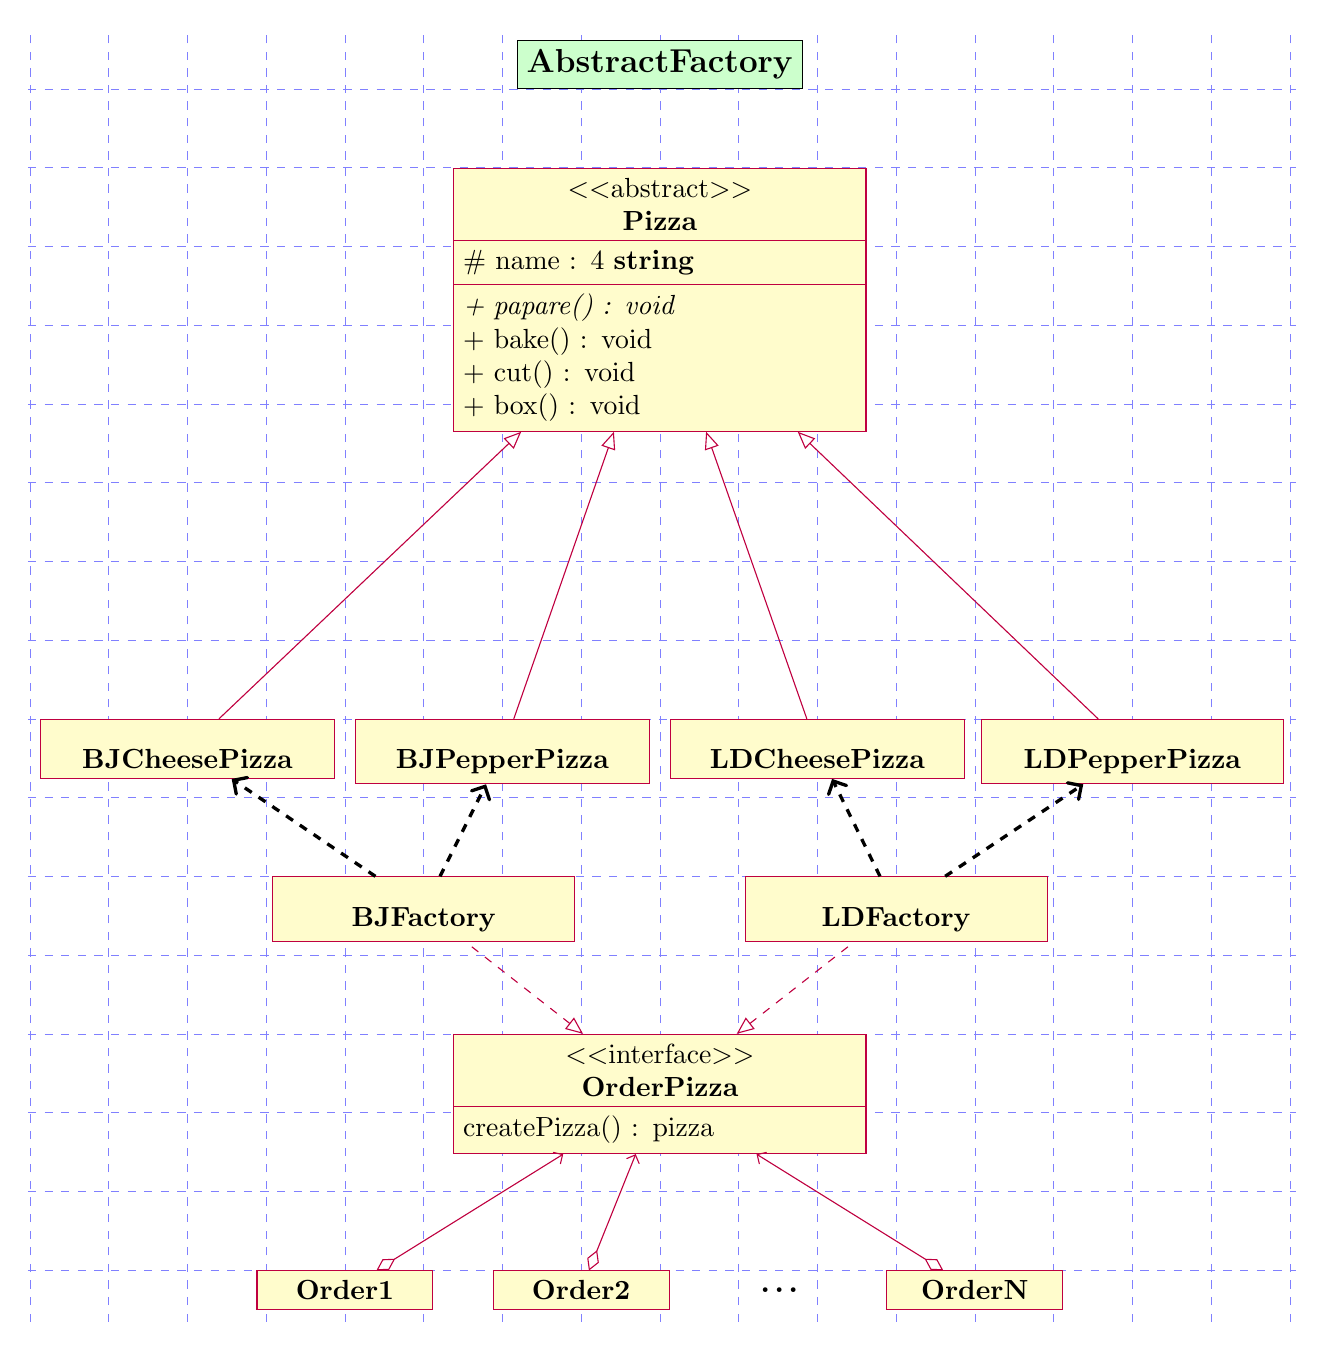
\begin{tikzpicture}[show background grid]
        \begin{abstractclass}{Pizza}{0,1}
            \attribute{\# name : \zihao{4} \textbf{string}}
            \operation[0]{+ papare() : void}
            \operation{+ bake() : void}
            \operation{+ cut() : void}
            \operation{+ box() : void}
        \end{abstractclass}
    	\begin{class}[text width=3.5cm, text height=.5cm]{BJCheesePizza}{-6,-6}
    		\inherit{Pizza}
    	\end{class}
		\begin{class}[text width=3.5cm, text height=.5cm]{BJPepperPizza}{-2,-6}
			\inherit{Pizza}
		\end{class}
        \begin{class}[text width=3.5cm, text height=.5cm]{LDCheesePizza}{2,-6}
    		\inherit{Pizza}
    	\end{class}
		\begin{class}[text width=3.6cm, text height=.5cm]{LDPepperPizza}{6,-6}
			\inherit{Pizza}
		\end{class}

		\begin{interface}{OrderPizza}{0, -10}
            \operation{createPizza() : pizza}
		\end{interface}
        
        \begin{class}[text width=3.6cm, text height=.5cm]{BJFactory}{-3,-8}
			\implement{OrderPizza}
		\end{class}
        \begin{class}[text width=3.6cm, text height=.5cm]{LDFactory}{3,-8}
			\implement{OrderPizza}
		\end{class}
	
		\node [draw, fill=green!20, above=1cm of Pizza] (title) {\large \textbf{AbstractFactory}};
	
		\draw[umlcd style dashed line, black,->, very thick] 
        (BJFactory) -- (BJCheesePizza);
        \draw[umlcd style dashed line, black,->, very thick] 
        (BJFactory) -- (BJPepperPizza);
        \draw[umlcd style dashed line, black,->, very thick] 
        (LDFactory) -- (LDCheesePizza);
        \draw[umlcd style dashed line, black,->, very thick] 
        (LDFactory) -- (LDPepperPizza);

        \begin{class}[text width=2cm]{Order1}{-4, -13}
        \end{class}
        \begin{class}[text width=2cm]{Order2}{-1, -13}
        \end{class}
        \begin{class}[text width=2cm]{OrderN}{4, -13}
        \end{class}
        \aggregation{Order1}{}{}{OrderPizza}
        \aggregation{Order2}{}{}{OrderPizza}
        \aggregation{OrderN}{}{}{OrderPizza}
        \node [right=of Order2] (OrderSlh){\huge ...};
    \end{tikzpicture}
\end{document}